%% ===== 5 Results =====
\section{Results}
\label{sec:results}

Counts below refer to the 49 papers of the main corpus; the two cross-language equivalence-detection papers (I3) are reported at the end of Section~\ref{sec:rq3}. A paper can use several oracles and several migration kinds, so columns do not sum to 49.

%% ---------------------------------------------------------------------
\subsection{Corpus overview}
\label{sec:overview}

The corpus grows quickly: \new{8 papers are from 2024, 14 from 2025 and 27 from 2026}\hcrev{, or 0.68\%, 0.98\% and 1.45\% of the papers scanned in each year (Table~\ref{tab:search}). The 2024 share may be slightly low, since 61 ICSE~2024 papers had no abstract and were matched on their titles only.}

Most papers are research-track (28), followed by industry/SEIP (\new{9}), journal-first (5), NIER (3), posters (2), \new{and one each in demonstrations and Ideas, Visions and Reflections (IVR). We call the NIER, IVR, demonstration and poster papers short papers.} Translation between languages dominates (XL, 33 papers), followed by library migration (LIB, 12), version migration (VER, 3), framework migration (FW, 3) and dialect translation (DIA, 2); 5 papers migrate legacy systems\hcrev{, as defined in Section~\ref{sec:background}}. Rust is a target language in 13 papers. The LLM is the proposed technique in 32 papers, the evaluated subject in 9, and both in 4; in the remaining 4 it is \hcrev{only a baseline (3, two of which propose a smaller neural model) or part of the evaluation tooling (1)}.

%% ---------------------------------------------------------------------
\subsection{RQ1: Which oracles are used?}
\label{sec:rq1}

Compilation and existing tests dominate; formal verification\hcrev{, LLM-generated tests} and LLM judges are rare (Figure~\ref{fig:oracle-freq}). \hcrev{We count an oracle when a paper reports its result on the final outputs, so the counts record which oracles papers use, not which ones their conclusions rest on.}

\begin{figure}[t]
  \centering
  %% Figure: oracle frequency in the 49 main-corpus papers (sheet "Mã hoá tổng hợp").
%% A paper can use several oracles, so bars do not sum to 49.
%% To change a number, edit both the bar value and its label [n (p%)].
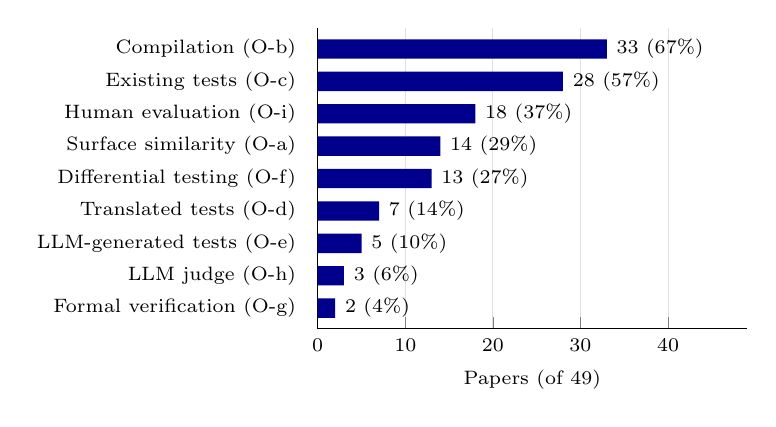
\begin{tikzpicture}
\begin{axis}[
  xbar, width=0.58\columnwidth, height=5.4cm, xmin=0, xmax=49, y dir=reverse,
  ytick=data, symbolic y coords={ob,oc,oi,oa,of,od,oe,oh,og},
  yticklabels={{Compilation (O-b)},{Existing tests (O-c)},{Human evaluation (O-i)},{Surface similarity (O-a)},{Differential testing (O-f)},{Translated tests (O-d)},{LLM-generated tests (O-e)},{LLM judge (O-h)},{Formal verification (O-g)}},
  yticklabel style={font=\scriptsize}, xticklabel style={font=\scriptsize},
  xtick={0,10,20,30,40}, xmajorgrids, grid style={gray!25}, axis lines*=left, ytick style={draw=none},
  bar width=7pt, enlarge y limits=0.08,
  point meta=explicit symbolic, nodes near coords, nodes near coords style={font=\scriptsize, anchor=west},
  xlabel={\scriptsize Papers (of 49)}, clip=false,
]
  \addplot[fill=blue!55!black, draw=none] coordinates {(33,ob) [33 (67\%)] (28,oc) [28 (57\%)] (18,oi) [18 (37\%)] (14,oa) [14 (29\%)] (13,of) [13 (27\%)] (7,od) [7 (14\%)] (5,oe) [5 (10\%)] (3,oh) [3 (6\%)] (2,og) [2 (4\%)]};
\end{axis}
\end{tikzpicture}

  \caption{\revtag Oracles used by the 49 main-corpus papers. A paper can use several oracles. \hcrev{An oracle is counted when the paper reports its result on the final outputs.}}
  \Description{Horizontal bar chart. Compilation 34 papers (69\%), existing tests 28 (57\%), human evaluation 17 (35\%), differential testing 14 (29\%), surface similarity 13 (27\%), translated tests 7 (14\%), LLM-generated tests 2 (4\%), LLM judge 2 (4\%), formal verification 2 (4\%).}
  \label{fig:oracle-freq}
\end{figure}

Most papers combine oracles: 9 use one, 17 use two, 17 use three, and 6 use four or more, up to \hcrev{five in RustAssure~\cite{rustassure}. Six of the 28 papers with existing tests report no compile rate, although their code must compile to run.} Nine papers use no oracle that executes code (none of O-c to O-f): they judge outputs by compilation, similarity, a human or an LLM. \hcrev{Five rely on a single oracle that does not run the code: 2 report only BLEU or CodeBLEU~\cite{vimpt,collaboration}, one only an LLM judge~\cite{wca4z}, and 2 only human judgment~\cite{pig,pli}.}
\TODO{O-b rule still open (reply to the response, V2). If RustRepoTrans and TransGraph lose O-b, compilation becomes 32 papers (65\%), 8 of the 28 papers with existing tests report no compile rate, and 11 papers use one oracle. If CAST gains O-b, compilation becomes 35 (71\%) and 5 of the 28 report no compile rate. Update Figure~\ref{fig:oracle-freq}, Tables~\ref{tab:cooc} and~\ref{tab:context} and this paragraph once the team decides.}

\begin{added}
Table~\ref{tab:cooc} shows which oracles are combined. Compilation accompanies most other oracles: \hcrev{22} of the 28 papers with existing tests also \new{use compilation as an oracle}, and so do \hcrev{12 of the 17} with human evaluation. Differential testing seldom appears next to existing tests (\hcrev{4 of 14} papers), and in \hcrev{9 of the 14} no \new{test-suite oracle} (O-c, O-d, O-e) is used. Both papers with formal verification also run differential tests.
\end{added}

\begin{table}[t]
  \centering
  \caption{\addedtag\revtag Oracle combinations in the main corpus. Each cell counts the papers that use both oracles; the diagonal gives the papers that use each oracle.}
  \label{tab:cooc}
  \footnotesize
  \setlength{\tabcolsep}{3.5pt}
  \begin{tabular}{@{}lrrrrrrrrr@{}}
    \toprule
        & O-a & O-b & O-c & O-d & O-e & O-f & O-g & O-h & O-i \\
    \midrule
    O-a & \hcrev{13} &  &  &  &  &  &  &  &  \\
    O-b & \hcrev{6} & \hcrev{34} &  &  &  &  &  &  &  \\
    O-c & \hcrev{7} & \hcrev{22} & 28 &  &  &  &  &  &  \\
    O-d & \hcrev{0} & 7 & 5 & 7 &  &  &  &  &  \\
    O-e & \hcrev{1} & \hcrev{1} & \hcrev{1} & \hcrev{0} & \hcrev{2} &  &  &  &  \\
    O-f & \hcrev{1} & \hcrev{12} & \hcrev{4} & 3 & \hcrev{0} & \hcrev{14} &  &  &  \\
    O-g & 0 & 2 & 0 & 1 & 0 & 2 & 2 &  &  \\
    O-h & \hcrev{0} & \hcrev{1} & \hcrev{0} & \hcrev{0} & \hcrev{0} & \hcrev{0} & 0 & \hcrev{2} &  \\
    O-i & \hcrev{4} & \hcrev{12} & \hcrev{6} & \hcrev{3} & \hcrev{0} & \hcrev{5} & 1 & \hcrev{1} & \hcrev{17} \\
    \bottomrule
  \end{tabular}
\end{table}

%% ---------------------------------------------------------------------
\subsection{RQ2: Where do oracles come from, and in which contexts?}
\label{sec:rq2}

\hcrev{Oracle use differs by context in this corpus (Table~\ref{tab:context}). Most groups are small, so patterns in groups of five papers or fewer are illustrative only.}

\begin{table*}[t]
  \centering
  \caption{\revtag Oracle use by context. Each cell counts papers in the group that use the oracle; $n$ is the group size. \new{IVR: Ideas, Visions and Reflections.}}
  \label{tab:context}
  \small
  \begin{tabular}{@{}lrrrrrrrrrr@{}}
    \toprule
    Group & $n$ & O-a & O-b & O-c & O-d & O-e & O-f & O-g & O-h & O-i \\
    \midrule
    Legacy                    & 5 & 0 & 1 & 0 & 0 & 1 & 2 & 0 & 1 & 1 \\
    Not legacy                & 44 & \hcrev{13} & \hcrev{33} & 28 & 7 & \hcrev{1} & \hcrev{12} & 2 & \hcrev{1} & \hcrev{16} \\
    \midrule
    XL                        & 33 & \hcrev{7} & \hcrev{22} & 20 & 6 & \hcrev{2} & \hcrev{11} & 2 & \hcrev{1} & \hcrev{6} \\
    LIB                       & 12 & 4 & 9 & 6 & 2 & 0 & 1 & 0 & 1 & 9 \\
    VER                       & 3 & 1 & 2 & 1 & 0 & 0 & 1 & 0 & 0 & 1 \\
    FW                        & 3 & 1 & 3 & 1 & 0 & 1 & 1 & 0 & 0 & 1 \\
    DIA                       & 2 & 1 & 1 & 0 & 0 & 0 & 1 & 0 & 0 & 2 \\
    \midrule
    Research                  & 28 & \hcrev{8} & 19 & 15 & 6 & \hcrev{1} & 8 & 2 & \hcrev{1} & \hcrev{13} \\
    Industry/SEIP             & 9 & 2 & 7 & 5 & 1 & \hcrev{1} & \hcrev{3} & 0 & 1 & 2 \\
    NIER, IVR, demo, poster   & 7 & 2 & 4 & 3 & 0 & 0 & 2 & 0 & 0 & 2 \\
    Journal-first             & 5 & 1 & \hcrev{4} & 5 & 0 & 0 & 1 & 0 & 0 & 0 \\
    \midrule
    2024                      & 8 & 3 & \hcrev{5} & 5 & 1 & 0 & 2 & 0 & 0 & 1 \\
    2025                      & 14 & 3 & 10 & 8 & 3 & 0 & 4 & 2 & 0 & 6 \\
    2026                      & 27 & \hcrev{7} & 19 & 15 & 3 & \hcrev{2} & \hcrev{8} & 0 & \hcrev{2} & \hcrev{10} \\
    \bottomrule
  \end{tabular}
\end{table*}

\begin{itemize}
  \item \textbf{\new{No legacy paper uses existing tests.}} Two of the 5 legacy papers run the original system as a differential oracle~\cite{kcobagent,coboljava}, one generates tests with an LLM from an extracted specification~\cite{ipmodern}, one uses an LLM judge~\cite{wca4z}, and one \new{compares the generated Java with the expected code by hand}~\cite{pli}. \hcrev{This is the one empty cell that chance does not easily explain: with 28 of the 49 papers using existing tests, about 3 legacy papers would be expected to use them. With five papers, all in the industry/SEIP or NIER tracks, legacy cannot be separated from track, and the result depends on our definition: if the three papers that call their C or Java sources legacy were flagged~\cite{evoc2rust,smartc2rust,codehints}, 2 of 8 legacy papers would use existing tests.}
  \item \textbf{\hcrev{Library migration often includes a human check.}} \new{Nine of the 12} LIB papers include human evaluation, against \hcrev{6} of 33 XL papers\hcrev{, but only 3 of these nine judge behavior without also running the code~\cite{pig,depupgrade,rulesynth}. Several human checks cover only part of the outputs, such as a 20\% sample of the patches that pass the tests~\cite{fruntke} or the 24 cases that have a developer's fix~\cite{bdupdater}.} No LIB paper uses LLM-generated tests or formal verification.
  \item \textbf{\hcrev{Both formal-verification papers target Rust}}~\cite{rustassure,vert}\hcrev{; with two papers, this is an observation rather than a pattern.}
  \item \textbf{\hcrev{LLM-based final-output oracles appear only in 2026.}} \hcrev{The 2 papers with LLM-generated tests~\cite{ipmodern,transagent} and the 2 with LLM judges~\cite{depupgrade,wca4z} are all from 2026. Earlier papers use LLM-generated tests only inside the technique~\cite{unitrans,collaboration}, and with four papers the timing may be chance.}
  \item \hcrev{\textbf{All 5 journal-first papers use existing tests}, and none uses human evaluation.}
  \item \textbf{\new{Zero cells}} mark combinations \new{that no paper uses}: legacy with \new{similarity,} existing, translated or formal-verification oracles; library migration with LLM-generated tests or formal verification; dialect translation with any \new{test-suite} oracle; and short papers with translated tests, generated tests, \new{formal verification} or LLM judges. \hcrev{Except for legacy with existing tests, each of these cells would hold at most 1.3 papers if oracle use did not depend on the group, so an empty cell says little on its own.}
\end{itemize}

\begin{added}
\paragraph{Where the ground truth comes from.} Table~\ref{tab:origin} breaks down the four execution-based oracles by the origin of their ground truth\hcrev{; we do not code the origin of the other oracles}. Existing tests split almost evenly: 14 papers use tests built for a benchmark of curated problems or reference translations, \new{12} use the test suite that a real project's developers wrote, and \new{2 use both~\cite{dgir,recodeagent}}. \hcrev{Among the 14 LIB and VER papers, 7 use existing tests, and 6 of these 7 rerun the client project's own suite after the change~\cite{pylibmig,byam,fruntke,bdupdater,googlemig,freshbrew}.} In translation between languages, benchmark tests are more common: 12 papers, against \new{6} with project suites and \new{2} with both.

Translated tests are mostly translated by the system under evaluation (5 of 7)\new{. In 4 of these papers a translation error can therefore affect the code and its tests alike; in IntentTester the migrated tests are themselves the output under evaluation}\hcrev{, so a pass shows that a migrated test passes on the target library, not that it still checks what the original test checked}\new{~\cite{intenttester}. In 3 papers the authors translated tests by hand, in one of them alongside tests translated by its system~\cite{lostintranslation,rustassure,recodeagent}.} \hcrev{Only 2 papers use LLM-generated tests in the sense of Table~\ref{tab:oracles}, where the expected outputs come from an LLM or a specification: one derives its tests from the same specification it uses to generate the code~\cite{ipmodern}, and one does not say where the expected outputs come from, which we code as O-e~\cite{transagent}. Tests that an LLM writes but whose expected outputs come from running the original are coded as differential testing (Section~\ref{sec:background}).} Differential testing takes its inputs from fuzzing, property-based testing or symbolic execution in 5 papers, reuses existing tests or benchmark data in 3, uses LLM-generated inputs in \hcrev{3~\cite{prognosticator,travel,recodeagent}}, compares curated samples or rendered screens in 2, and does not describe its inputs in 2\hcrev{; one paper has two input origins~\cite{recodeagent}}.
\end{added}

\begin{table}[t]
  \centering
  \caption{\addedtag\revtag Where the ground truth of execution-based oracles comes from (main corpus). Per-paper codes are in Appendix~\ref{app:primary}. \new{$^{*}$One paper uses both translated-test origins, so the O-d rows sum to 8.} \hcrev{One differential-testing paper has two input origins, so the O-f rows sum to 15. Origin is coded only for these four oracles.}}
  \label{tab:origin}
  \small
  \begin{tabular}{@{}P{0.8\linewidth}r@{}}
    \toprule
    Oracle and origin & Papers \\
    \midrule
    \multicolumn{2}{@{}l}{\textit{O-c Existing tests (28)}} \\
    \quad Built for a benchmark (curated problems, reference translations) & 14 \\
    \quad A real project's own test suite & 12 \\
    \quad Both & 2 \\
    \multicolumn{2}{@{}l}{\textit{O-d Translated tests (7)}} \\
    \quad Translated by the system under evaluation & 5 \\
    \quad Translated by hand by the authors\new{\textsuperscript{*}} & 3 \\
    \multicolumn{2}{@{}l}{\textit{O-e LLM-generated tests (\hcrev{2})}} \\
    \quad Derived from the specification that also generates the code & 1 \\
    \quad Source of expected outputs not stated & 1 \\
    \multicolumn{2}{@{}l}{\textit{O-f Differential testing (\hcrev{14})}} \\
    \quad Inputs from fuzzing, property-based testing or symbolic execution & 5 \\
    \quad Inputs from existing tests or benchmark data & 3 \\
    \quad Inputs generated by an LLM & \hcrev{3} \\
    \quad Curated samples or rendered screens & 2 \\
    \quad Inputs not described & 2 \\
    \bottomrule
  \end{tabular}
\end{table}

%% ---------------------------------------------------------------------
\subsection{RQ3: Threats to oracle reliability}
\label{sec:rq3}

\paragraph{Oracle disagreement.} \new{Thirty-three} papers apply two or more oracles to the same outputs and report \new{numbers under each in the text or tables. A few more apply several oracles but report them only as a combined rate~\cite{byam}, a pass/fail summary~\cite{ipmodern,deepmodelx}, a chart~\cite{transgraph}, or not separately~\cite{googlemig}.} The largest and most consistent gap is between compiling and behaving correctly\new{: 18 papers report both a compile rate (or the rate of another well-formedness check) and a behavioral pass rate for the same outputs, and in every configuration plotted in Figure~\ref{fig:compile-gap} behavior trails compilation, by 3 to 98 percentage points}.

\begin{figure}[t]
  \centering
  %% Figure: compile rate vs behavioral pass rate in the 18 papers that report both
%% for the same outputs (recount 25/10/2026, revised after an independent check;
%% sheet "Mã hoá tổng hợp", column "Nhiều oracle trên cùng output", group "Hình 3";
%% numbers from field 6 of "Trích xuất (nháp)", checked against the papers).
%% Each row: (compile rate, behavioral pass rate) as reported; rows sorted by gap.
%% Fractions used: DepUpgrade 119/123 and 62/123 (equivalent patches over all
%% tasks); Fruntke & Krinke 40/65 and 12/65; VERT 539/569 and 295/569;
%% IntentTester 2,776/3,257 and 1,996/3,257; RISE 136/143 and 124/143;
%% Translation Tag Team 274/350 and 253/350; BatFix 605/698 and 567/698.
%% If a value changes, edit it here AND the gap label on the right.
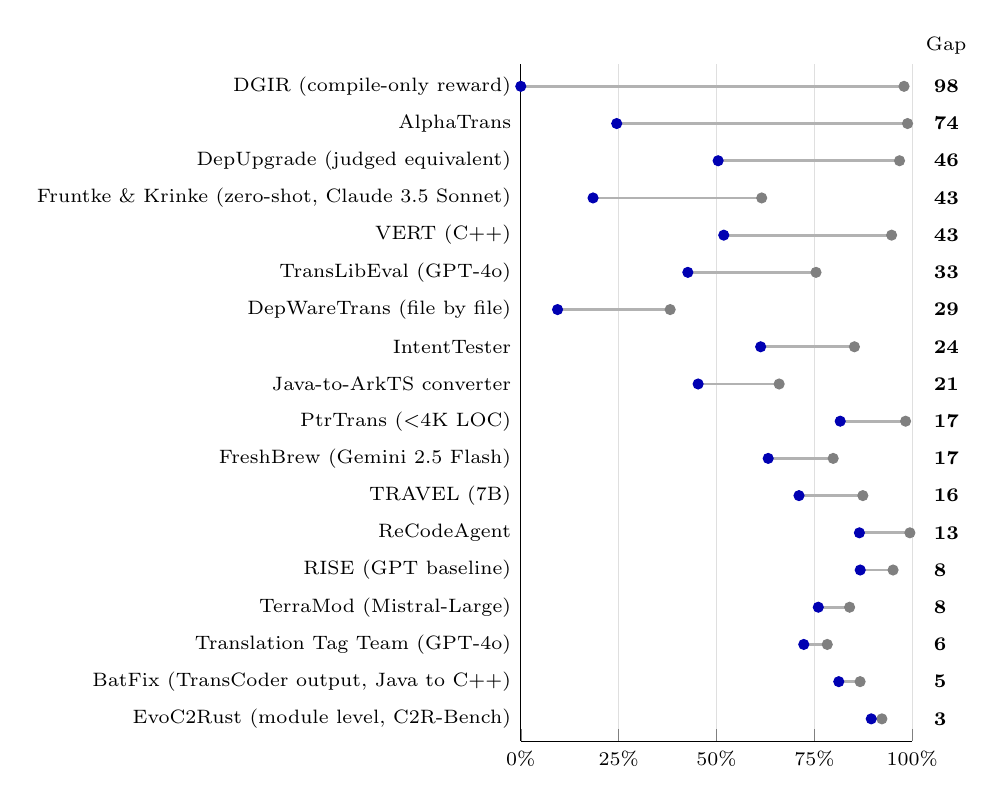
\begin{tikzpicture}
\begin{axis}[
  scale only axis, width=0.41\columnwidth, height=8.6cm,
  xmin=0, xmax=100, ymin=0.4, ymax=18.6, y dir=reverse,
  ytick={1,...,18}, yticklabels={{DGIR (compile-only reward)},{AlphaTrans},{DepUpgrade (judged equivalent)},{Fruntke \& Krinke (zero-shot, Claude 3.5 Sonnet)},{VERT (C++)},{TransLibEval (GPT-4o)},{DepWareTrans (file by file)},{IntentTester},{Java-to-ArkTS converter},{PtrTrans ($<$4K LOC)},{FreshBrew (Gemini 2.5 Flash)},{TRAVEL (7B)},{ReCodeAgent},{RISE (GPT baseline)},{TerraMod (Mistral-Large)},{Translation Tag Team (GPT-4o)},{BatFix (TransCoder output, Java to C++)},{EvoC2Rust (module level, C2R-Bench)}},
  yticklabel style={font=\scriptsize}, xticklabel style={font=\scriptsize},
  xtick={0,25,50,75,100}, xticklabel={\pgfmathprintnumber{\tick}\%},
  xmajorgrids, grid style={gray!25}, axis lines*=left, ytick style={draw=none},
  clip=false,
]
  \draw[gray!60, line width=1pt] (axis cs:0.00,1) -- (axis cs:97.90,1);
  \draw[gray!60, line width=1pt] (axis cs:24.50,2) -- (axis cs:98.80,2);
  \draw[gray!60, line width=1pt] (axis cs:50.41,3) -- (axis cs:96.75,3);
  \draw[gray!60, line width=1pt] (axis cs:18.46,4) -- (axis cs:61.54,4);
  \draw[gray!60, line width=1pt] (axis cs:51.85,5) -- (axis cs:94.73,5);
  \draw[gray!60, line width=1pt] (axis cs:42.67,6) -- (axis cs:75.42,6);
  \draw[gray!60, line width=1pt] (axis cs:9.39,7) -- (axis cs:38.16,7);
  \draw[gray!60, line width=1pt] (axis cs:61.28,8) -- (axis cs:85.23,8);
  \draw[gray!60, line width=1pt] (axis cs:45.30,9) -- (axis cs:66.00,9);
  \draw[gray!60, line width=1pt] (axis cs:81.60,10) -- (axis cs:98.30,10);
  \draw[gray!60, line width=1pt] (axis cs:63.20,11) -- (axis cs:79.80,11);
  \draw[gray!60, line width=1pt] (axis cs:71.07,12) -- (axis cs:87.38,12);
  \draw[gray!60, line width=1pt] (axis cs:86.50,13) -- (axis cs:99.40,13);
  \draw[gray!60, line width=1pt] (axis cs:86.71,14) -- (axis cs:95.10,14);
  \draw[gray!60, line width=1pt] (axis cs:76.00,15) -- (axis cs:84.00,15);
  \draw[gray!60, line width=1pt] (axis cs:72.29,16) -- (axis cs:78.29,16);
  \draw[gray!60, line width=1pt] (axis cs:81.23,17) -- (axis cs:86.68,17);
  \draw[gray!60, line width=1pt] (axis cs:89.53,18) -- (axis cs:92.25,18);
  \addplot[only marks, mark=*, mark size=1.8pt, color=gray] coordinates {(97.90,1) (98.80,2) (96.75,3) (61.54,4) (94.73,5) (75.42,6) (38.16,7) (85.23,8) (66.00,9) (98.30,10) (79.80,11) (87.38,12) (99.40,13) (95.10,14) (84.00,15) (78.29,16) (86.68,17) (92.25,18)};
  \addplot[only marks, mark=*, mark size=1.8pt, color=blue!70!black] coordinates {(0.00,1) (24.50,2) (50.41,3) (18.46,4) (51.85,5) (42.67,6) (9.39,7) (61.28,8) (45.30,9) (81.60,10) (63.20,11) (71.07,12) (86.50,13) (86.71,14) (76.00,15) (72.29,16) (81.23,17) (89.53,18)};
  \node[anchor=west, font=\scriptsize\bfseries] at (axis cs:103,1) {98};
  \node[anchor=west, font=\scriptsize\bfseries] at (axis cs:103,2) {74};
  \node[anchor=west, font=\scriptsize\bfseries] at (axis cs:103,3) {46};
  \node[anchor=west, font=\scriptsize\bfseries] at (axis cs:103,4) {43};
  \node[anchor=west, font=\scriptsize\bfseries] at (axis cs:103,5) {43};
  \node[anchor=west, font=\scriptsize\bfseries] at (axis cs:103,6) {33};
  \node[anchor=west, font=\scriptsize\bfseries] at (axis cs:103,7) {29};
  \node[anchor=west, font=\scriptsize\bfseries] at (axis cs:103,8) {24};
  \node[anchor=west, font=\scriptsize\bfseries] at (axis cs:103,9) {21};
  \node[anchor=west, font=\scriptsize\bfseries] at (axis cs:103,10) {17};
  \node[anchor=west, font=\scriptsize\bfseries] at (axis cs:103,11) {17};
  \node[anchor=west, font=\scriptsize\bfseries] at (axis cs:103,12) {16};
  \node[anchor=west, font=\scriptsize\bfseries] at (axis cs:103,13) {13};
  \node[anchor=west, font=\scriptsize\bfseries] at (axis cs:103,14) {8};
  \node[anchor=west, font=\scriptsize\bfseries] at (axis cs:103,15) {8};
  \node[anchor=west, font=\scriptsize\bfseries] at (axis cs:103,16) {6};
  \node[anchor=west, font=\scriptsize\bfseries] at (axis cs:103,17) {5};
  \node[anchor=west, font=\scriptsize\bfseries] at (axis cs:103,18) {3};
  \node[anchor=west, font=\scriptsize] at (axis cs:101,-0.1) {Gap};
\end{axis}
\end{tikzpicture}

  \caption{\new{Share of outputs passing compilation or another well-formedness check (gray) versus behavioral pass rate (blue) in the 18 papers that report both for the same outputs, with the gap in percentage points. Numbers are as reported in each paper, for the configuration named in parentheses and otherwise for the paper's own system; the DGIR row is its compile-only-reward ablation, the RISE row its GPT-based LLM baseline, \new{the DepWareTrans row a file-by-file baseline, and the BatFix row the translations before repair}. The behavioral oracle differs by paper.}}
  \Description{Dot plot with one row per paper. Gaps range from 98 percentage points for the DGIR ablation (97.9\% compile, 0\% correct) to 3 percentage points for EvoC2Rust (92.25\% versus 89.53\%).}
  \label{fig:compile-gap}
\end{figure}

Other disagreements involve surface similarity and test strength (Table~\ref{tab:disagree}). \new{Besides the 18 papers in Figure~\ref{fig:compile-gap} and 6 more in Table~\ref{tab:disagree}, the other 9 papers report numbers under several oracles in \new{other forms}: counts of compile errors next to test pass rates~\cite{smartc2rust}, \new{breakdowns of failures by stage~\cite{lostintranslation,rustrepotrans}, a compile rate per function next to equivalence per return value~\cite{rustassure},} bugs found by each checking stage~\cite{prognosticator}, build errors next to diff similarity~\cite{codeplan}, rendered-screen similarity next to structural similarity~\cite{guimigrator}, a manual review of outputs that failed an AST match~\cite{rulesynth}, \new{and a syntax-check rate next to a correctness rate from matching and manual review~\cite{pylibmig}}.}

\begin{table*}[t]
  \centering
  \caption{Other oracle disagreements reported on the same outputs\new{. TerraMod and VERT also appear in Figure~\ref{fig:compile-gap}. CA: computational accuracy, the share of outputs that pass the tests}.}
  \label{tab:disagree}
  \small
  \begin{tabular}{@{}P{0.22\linewidth} P{0.25\linewidth} P{0.45\linewidth}@{}}
    \toprule
    Paper & Oracles compared & Result \\
    \midrule
    UniTrans~\cite{unitrans} & Tests (CA) vs exact match & 87.92\% vs 18.04\% \new{(GPT-3.5)} \\
    CAST~\cite{cast} & Tests (CA) vs exact match & 69.72\% vs 16.23\% (GPT-4o) \\
    TransAgent~\cite{transagent} & Tests (CA) vs CodeBLEU & TransCoder Python to Java: CA 2.4\%, CodeBLEU 40.1 \\
    TerraMod~\cite{terramod} & Execution (Pass@1) vs CrystalBLEU & \new{LLaMA-4-Maverick:} baseline 44\% / 0.78 vs TerraMod 76\% / 0.66\new{; the two metrics rank the systems in opposite order (one of four models)} \\
    VERT~\cite{vert} & Compile, property-based tests, bounded and full verification & C++, 569 programs: 539, 295, 233 and 19 pass \\
    MBTA~\cite{mbta} & Tests (CA) vs mutation-based score & 168 programs reach perfect CA, yet TransCoder mistranslates at least one of their mutants \\
    BDUpdater~\cite{bdupdater} & Existing tests vs developer's fix & 1 of 24 adaptations passes the tests but is not equivalent \\
    Code hints~\cite{codehints} & Fuzzing check vs manual review & Symbolic engine without hints: 23 candidates pass the check, 7 are correct \\
    \bottomrule
  \end{tabular}
\end{table*}

Three patterns recur: compiling says little about equivalence; surface similarity can rank systems in the opposite order to execution; and \new{tests and fuzzing checks miss faults that mutation analysis, verification or human review find}.

\paragraph{\new{Limitations that studies report.}} We grouped the oracle limitations that papers state about their own evaluation (Table~\ref{tab:limits}).

\begin{table}[t]
  \centering
  \caption{Oracle limitations that papers state about their own evaluation. \new{Each paper is counted once, under its main theme.}}
  \label{tab:limits}
  \small
  \begin{tabular}{@{}P{0.8\linewidth}r@{}}
    \toprule
    Theme & Papers \\
    \midrule
    Weak or few tests, so passing tests does not imply equivalence & 15 \\
    Incomplete differential, fuzzing, symbolic or bounded checks & 6 \\
    Subjective human evaluation, or no agreement measured & 4 \\
    The LLM games the oracle: optimizes for compiling or passing tests & 3 \\
    Oracle derived from the same source as the output (tests and code generated from one specification) & 3 \\
    Misleading surface similarity & 3 \\
    Compiling does not imply correct behavior & 2 \\
    No executable oracle available & 2 \\
    \new{A limitation of the oracle unrelated to equivalence (e.g., readability)} & 2 \\
    \midrule
    No limitation of the paper's own oracle stated & 9 \\
    \bottomrule
  \end{tabular}
\end{table}

Test weakness is the most \new{common main} limitation \new{(15 papers), even though existing tests remain the second most used oracle (28 papers)}. Nine papers state \new{no limitation of} their own oracle, including both BLEU-only papers and the paper that relies only on an LLM judge. Oracle gaming is a new theme: a model rewarded for compiling emits trivial code such as \texttt{panic!}~\cite{dgir}, an LLM rewrites code until tests pass~\cite{smartc2rust}, and benchmark agents \new{game the tests, which FreshBrew detects with a coverage threshold}~\cite{freshbrew}.

\begin{added}
\paragraph{Oracles reused inside the technique.} \new{Although we code only the oracle that judges the final output (Section~\ref{sec:extraction}),} in some papers the same oracle also selects or repairs the outputs it later judges. InterTrans stops its search as soon as a candidate passes the benchmark tests and reports accuracy on those same tests~\cite{intertrans}; SmartC2Rust runs the same tests in its repair loop and as its final measure~\cite{smartc2rust}; and RISE uses its differential check both as a validity step inside the technique and as the evaluation~\cite{rise}. In these 3 papers the reported pass rate shows that the output satisfies the oracle it was selected against, not that it is equivalent; a held-out oracle would separate the two. Two further papers train \new{their models} against the same kind of oracle they report, \new{though not necessarily on the evaluated problems}: TRAVEL rewards its model with LLM-generated test components of the kind it also evaluates with~\cite{travel}, and \new{DGIR, in an ablation that rewards compilation only, shows where this leads (Figure~\ref{fig:compile-gap})}~\cite{dgir}. We flagged these cases during extraction rather than coding them systematically, so there may be more.
\end{added}

\paragraph{Cross-language equivalence detection (I3).} Two papers form the separate tier. One measures how well LLMs judge whether code in two languages is equivalent: GPT-3.5-Turbo reaches F1 0.99 on XLCoST but 0.82 on CodeNet~\cite{moumoula}, which is direct evidence on LLMs as oracles (O-h). The other checks equivalence formally between C++ or PyTorch specifications and Chisel or Verilog implementations through MLIR, without an LLM~\cite{equivfusion}: a kind of formal cross-language oracle that the software translation papers in our corpus barely use.
